\documentclass{article}
% Chinese
% \documentclass[UTF8, nofonts, mathptmx, 12pt, onecolumn]{article}
% \usepackage{xeCJK}
% \setCJKmainfont{SimSun}
\usepackage{amsmath}
\usepackage{amsfonts}
\usepackage{amssymb}
\usepackage{wasysym}
% \usepackage{ctex}
\usepackage{graphicx}
\usepackage{float}
\usepackage{geometry}
\geometry{a4paper,scale=0.8}
\usepackage{caption}
\usepackage{subcaption}
% \newcommand{\oiint}{\mathop{{\int\!\!\!\!\!\int}\mkern-21mu \bigcirc} {}}
\newcommand*{\dif}{\mathop{}\!\mathrm{d}}
\newcommand*{\md}{\mathop{}\!\mathrm{d}}
\newcommand*{\me}{\mathrm{e}}

% \usepackage{parskip}
% \setlength{\parindent}{0cm}

\usepackage{bm}
\let\Oldmathbf\mathbf
\renewcommand{\mathbf}[1]{\boldsymbol{\Oldmathbf{#1}}}
\let\eqnarray\align

\renewcommand*{\arraystretch}{2}
\usepackage{units}
\renewcommand{\frac}{\nicefrac}

\usepackage{cellspace}
\setlength{\cellspacetoplimit}{5pt}
\setlength{\cellspacebottomlimit}{5pt}


\author{Xiping Hu}
\usepackage{authblk}
\author{Xiping Hu}
\affil{https://hxp.plus/}
\title{Homework for Chapter 7}

\begin{document}
\maketitle

\begin{figure}[H]
  \centering
  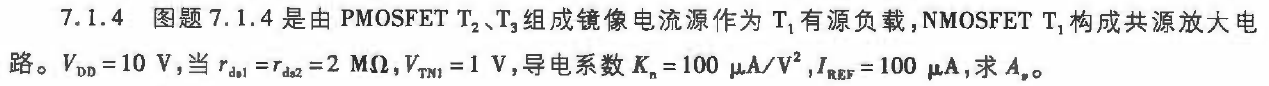
\includegraphics[width=\linewidth]{figures/Problem714} 
  \label{fig:}
\end{figure}

\begin{figure}[H]
  \centering
  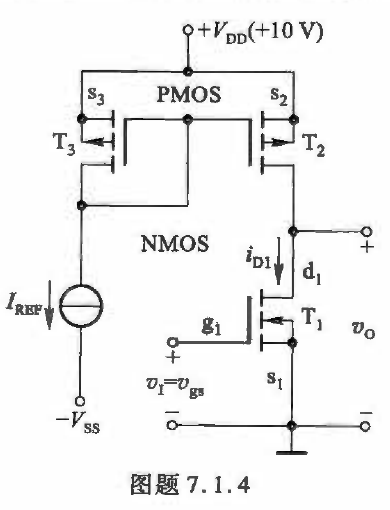
\includegraphics[width=0.4\linewidth]{figures/Problem7141} 
  \label{fig:}
\end{figure}

\begin{figure}[H]
  \centering
  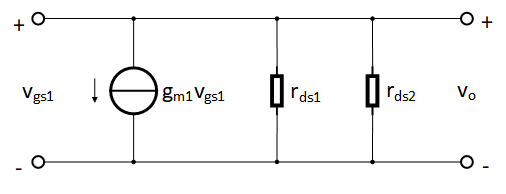
\includegraphics[width=0.8\linewidth]{figures/Problem7142} 
  \label{fig:}
\end{figure}

\begin{equation*}
  \begin{aligned}
    g_{m1} = 2 K_n \left( v_{GS1} - V_{TN1} \right) = 2 K_n \sqrt{\dfrac{I_{D1}}{K_n} } = 200 \  \mathrm{\mu S}
  \end{aligned}
\end{equation*}

\begin{equation*}
  \begin{aligned}
    A_v = \dfrac{v_o}{v_i} = - \dfrac{g_m v_{gs} \left( r_{ds1} \parallel r_{ds2} \right)}{v_{gs}} = - 200 
  \end{aligned}
\end{equation*}





\end{document}